\documentclass[10pt]{article}

\usepackage{spheric}
%%%TITLE
\title{An SPH numerical wave-current tank}
\date{}

%%AFFILIATIONS

\author[$\relax$]{Ming HE}
\author[$\relax$]{Hongshu WANG}
\author[$\relax$]{Xifeng GAO$^\dagger$}
\author[$\relax$]{Wanhai XU}
\author[$\relax$]{Yang SHI}
\affil[$\relax$]{The State Key Laboratory of Hydraulic Engineering Simulation and Safety, Tianjin University, Tianjin, China}

\affil[$\relax$]{\email{\dagger}{gaoxifeng@tju.edu.cn}}


%%DOCUMENT
\begin{document}

\maketitle

%\SelectedTopics{}

%%PLEASE PUT YOUR ABSTRACT HERE
\begin{abstract}
Numerical simulation of wave-current-structure interaction is of great value to coastal and ocean engineering, and is heavily dependent on the state of the art of the numerical wave-current tank (hereinafter denoted as ``NWCT''). Up to now, NWCT has been successfully established based on conventional Eulerian methods. But for Lagrangian method, it still lies in the stage of wave-structure interaction or current-structure interaction.

In this paper, the SPH method is extended to build a NWCT for the first time. The propagation wave is generated by a piston-type wave-maker set at the upstream end of the tank. At the other end, an artificial damping layer is arranged to absorb the outgoing wave. An inflow region and a symmetrical outflow region are set below the bottom of the tank, lying on the opposite sides but between the wave-maker and damping layer. By imposing a constant velocity and the hydrostatic pressure in these two regions together with a cyclic boundary condition, the desired uniform current is implemented. In addition, two approaches are used to accelerate the stabilization of the flow field. One is applying a ramp function to the particle velocity in the inflow and outflow regions. The other is employing a temporary ``rigid-lid treatment'' to the fluid particles close to the water surface. In other words, the vertical positions and velocities of these near-surface particles are restricted, while their horizontal components are free. The former approach buffers the jet flow at the inlet and accordingly weakens the unnecessary sound wave. The latter approach reduces the quasi ``U''-tube effect caused by the variations of surface elevation above the inlet and outlet. Thus, the simulation duration is shortened at least fivefold.

To validate the proposed model, a test case of surface wave following a current in a constant water depth is conducted. The calculated water surface profile and velocity distribution covering the whole water depth are compared with the experimental data of Umeyama \cite{umeyama2010coupled} in Figure \ref{fig:53}. The favourable agreement demonstrates that the established NWCT based on SPH method is capable of accurately reproducing wave-current coupling. 

\begin{figure}[!htb]
\centering
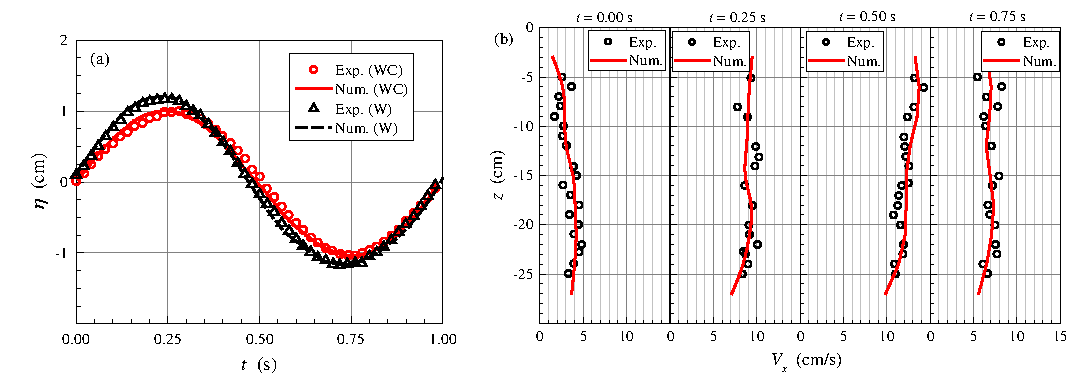
\includegraphics[width=0.95\textwidth]{53-1.pdf}
\caption{Comparison of numerical and experimental (a) wave surface profile and (b) horizontal-velocity distribution}\label{fig:53}
\end{figure}

\end{abstract}


%%THE END OF ABSTRACT

\addbib

\end{document}
